%----------
%   WARNING
%----------

% This Guide contains Library recommendations based mainly on APA and IEEE styles, but you must always follow the guidelines of your TFG Tutor and the TFG regulations for your degree.

% THIS TEMPLATE IS BASED ON THE IEEE STYLE 


%----------
% DOCUMENT SETTINGS
%----------

\documentclass[12pt]{report} % font: 12pt

% margins: 2.5 cm top and bottom; 3 cm left and right
\usepackage[
a4paper,
vmargin=2.5cm,
hmargin=3cm
]{geometry}

% Paragraph Spacing and Line Spacing: Narrow (6 pt / 1.15 spacing) or Moderate (6 pt / 1.5 spacing)
\renewcommand{\baselinestretch}{1.15}
\parskip=6pt

% Color settings for cover and code listings 
\usepackage[table]{xcolor}
\definecolor{azulUC3M}{RGB}{0,0,102}
\definecolor{gray97}{gray}{.97}
\definecolor{gray75}{gray}{.75}
\definecolor{gray45}{gray}{.45}

% PDF/A -- Important for its inclusion in e-Archive. PDF/A is the optimal format for preservation and for the generation of metadata: http://uc3m.libguides.com/ld.php?content_id=31389625. 

% In the template we include the file OUTPUT.XMPDATA. You can download that file and include the metadata that will be incorporated into the PDF file when you compile the memoria.tex file. Then upload it back to your project.  
\usepackage[a-1b]{pdfx}

% LINKS
\usepackage{hyperref}
\hypersetup{colorlinks=true,
	linkcolor=black, % links to parts of the document (e.g. index) in black
	urlcolor=blue} % links to resources outside the document in blue

% MATH EXPRESSIONS
\usepackage{amsmath,amssymb,amsfonts,amsthm}

% Character encoding
\usepackage{txfonts} 
\usepackage[T1]{fontenc}
\usepackage[utf8]{inputenc}

% English settings
\usepackage[english]{babel} 
\usepackage[babel, english=american]{csquotes}
\AtBeginEnvironment{quote}{\small}

% Footer settings
\usepackage{fancyhdr}
\pagestyle{fancy}
\fancyhf{}
\renewcommand{\headrulewidth}{0pt}
\rfoot{\thepage}
\fancypagestyle{plain}{\pagestyle{fancy}}

% DESIGN OF THE TITLES of the parts of the work (chapters and epigraphs or sub-chapters)
\usepackage{titlesec}
\usepackage{titletoc}
\titleformat{\chapter}[block]
{\large\bfseries\filcenter}
{\thechapter.}
{5pt}
{\MakeUppercase}
{}
\titlespacing{\chapter}{0pt}{0pt}{*3}
\titlecontents{chapter}
[0pt]                                               
{}
{\contentsmargin{0pt}\thecontentslabel.\enspace\uppercase}
{\contentsmargin{0pt}\uppercase}                        
{\titlerule*[.7pc]{.}\contentspage}                 

\titleformat{\section}
{\bfseries}
{\thesection.}
{5pt}
{}
\titlecontents{section}
[5pt]                                               
{}
{\contentsmargin{0pt}\thecontentslabel.\enspace}
{\contentsmargin{0pt}}
{\titlerule*[.7pc]{.}\contentspage}

\titleformat{\subsection}
{\normalsize\bfseries}
{\thesubsection.}
{5pt}
{}
\titlecontents{subsection}
[10pt]                                               
{}
{\contentsmargin{0pt}                          
	\thecontentslabel.\enspace}
{\contentsmargin{0pt}}                        
{\titlerule*[.7pc]{.}\contentspage}  


% Tables and figures settings
\usepackage{multirow} % combine cells 
\usepackage{caption} % customize the title of tables and figures
\usepackage{floatrow} % we use this package and its \ ttabbox and \ ffigbox macros to align the table and figure names according to the defined style.
\usepackage{array} % with this package we can define in the following line a new type of column for tables: custom width and centered content
\newcolumntype{P}[1]{>{\centering\arraybackslash}p{#1}}
\DeclareCaptionFormat{upper}{#1#2\uppercase{#3}\par}
\usepackage{graphicx}
\graphicspath{{imagenes/}} % Images folder

% Table layout for engineering
\captionsetup*[table]{
	format=upper,
	name=TABLE,
	justification=centering,
	labelsep=period,
	width=.75\linewidth,
	labelfont=small,
	font=small
}

% Figures layout for engineering
\captionsetup[figure]{
	format=hang,
	name=Fig.,
	singlelinecheck=off,
	labelsep=period,
	labelfont=small,
	font=small		
}

% FOOTNOTES
\usepackage{chngcntr} % continuous numbering of footnotes
\counterwithout{footnote}{chapter}

% CODE LISTINGS 
% support and styling for listings. More information in  https://es.wikibooks.org/wiki/Manual_de_LaTeX/Listados_de_código/Listados_con_listings
\usepackage{listings}

% Custom listing
\lstdefinestyle{estilo}{ frame=Ltb,
	framerule=0pt,
	aboveskip=0.5cm,
	framextopmargin=3pt,
	framexbottommargin=3pt,
	framexleftmargin=0.4cm,
	framesep=0pt,
	rulesep=.4pt,
	backgroundcolor=\color{gray97},
	rulesepcolor=\color{black},
	%
	basicstyle=\ttfamily\footnotesize,
	keywordstyle=\bfseries,
	stringstyle=\ttfamily,
	showstringspaces = false,
	commentstyle=\color{gray45},     
	%
	numbers=left,
	numbersep=15pt,
	numberstyle=\tiny,
	numberfirstline = false,
	breaklines=true,
	xleftmargin=\parindent
}

\captionsetup*[lstlisting]{font=small, labelsep=period}
 
\lstset{style=estilo}
\renewcommand{\lstlistingname}{\uppercase{Código}}


% REFERENCES 

% IEEE bibliography setup
\usepackage[backend=biber, style=ieee, isbn=false,sortcites, maxbibnames=6, minbibnames=1]{biblatex} % Setting for IEEE citation style, recommended for engineering. "maxbibnames" indicates that from 6 authors truncate the list in the first one (minbibnames) and add "et al." as used in the IEEE style.

\addbibresource{referencias.bib} % The references.bib file in which the bibliography used should be


%-------------
%	DOCUMENT
%-------------

\begin{document}
\pagenumbering{roman} % Roman numerals are used in the numbering of the pages preceding the body of the work.
	
%----------
%	COVER
%----------	
\begin{titlepage}
	\begin{sffamily}
	\color{azulUC3M}
	\begin{center}
		\begin{figure}[H] % UC3M Logo
			\makebox[\textwidth][c]{
\includegraphics[width=16cm]{logo_UC3M.png}}
		\end{figure}
		\vspace{2.5cm}
		\begin{Large}
			Degree in Data Science and Engineering\\
            Double Degree in Telecommunications Engineering and Data Science and Engineering\\
			 2024-2025\\ % Academic year
			\vspace{2cm}		
			\textsl{Data Science Project Midterm Report}
			\bigskip
			
		\end{Large}
		 	{\Huge Financial Transaction Fraud Detection: Securing the Industry with Artificial Intelligence}\\
		 	\vspace*{0.5cm}
	 		\rule{10.5cm}{0.1mm}\\
			\vspace*{0.5cm}
		\begin{Large}
			Silvia Diez\\
			Andrea López \\
            César Ramírez \\
            Enica King \\ 
            Emma Hernández 
            \\
		\end{Large}
	\end{center}
	\vfill
	\color{black}
	% IF OUR WORK IS TO BE PUBLISHED UNDER A CREATIVE COMMONS LICENSE, INCLUDE THESE LINES. IS THE RECOMMENDED OPTION.
	
\includegraphics[width=4.2cm]{creativecommons.png}\\ % Creative Commons Logo
    This work is licensed under Creative Commons \textbf{Attribution – Non Commercial – Non Derivatives}
	\end{sffamily}
\end{titlepage}


%----------
%	Table of Contents (TOC)
%----------	

%--
% TOC
%-
\tableofcontents
\thispagestyle{fancy}


%--
% List of figures. If they are not included, comment the following lines
% %-
% \listoffigures
% \thispagestyle{fancy}


% %--
% % List of tables. If they are not included, comment the following lines
% %-
% \listoftables
% \thispagestyle{fancy}

%----------
%	DEDICATION
%----------	

% \chapter{Dedication}
% This project would not have been possible without our supervising professor Fco. Javier Nogales, the coordinating professor Fernando Díaz de María, and the team at Bluetab: María Angeles Quesada, Juan Francisco Huete, and Cruz Mateo. 

%----------
%	THESIS
%----------	
\clearpage
\pagenumbering{arabic} % numbering with Arabic numerals for the rest of the document.	


\chapter{Introduction}
\section{Summary}
This project is a collaboration between the IBM company Bluetab and  students of the Charles III of Madrid University for the Data Science Project class. Providing students with professional mentorship allowed for application of theoretical concepts to a project in a professional context. Over the course of four months, these main four tasks were carried out: data pre-processing, development of a technical solution, analysis of legal and ethical aspects and analysis of the economic feasibility of the proposed solution.

\section{Objectives}
The main goals of the project were to use advanced Machine Learning (ML) techniques in order to accurately classify cases of financial fraud. Doing so would improve the detection capacity of illegal activity, minimize economic losses, and strengthen banking and insurance by securing financial operations.

\section{Initial Obstacles}
In the first phases of the project, making the connection between the task at hand and the datasets provided by the Bluetab team was the biggest hurdle to overcome. The datasets contained uninterpretable variables, misleading columns, and class imbalances that required a great effort in the preprocessing stage. Furthermore, establishing our working methods and workflow was also difficult since this project needed more documentation and organization than any previous project, and our groupmates and topic were assigned rather than freely chosen.

\section{Timeline}
Key events of the project are mapped out below; meetings with the company and with team members have not been listed.
\begin{figure}[H]
    \centering
    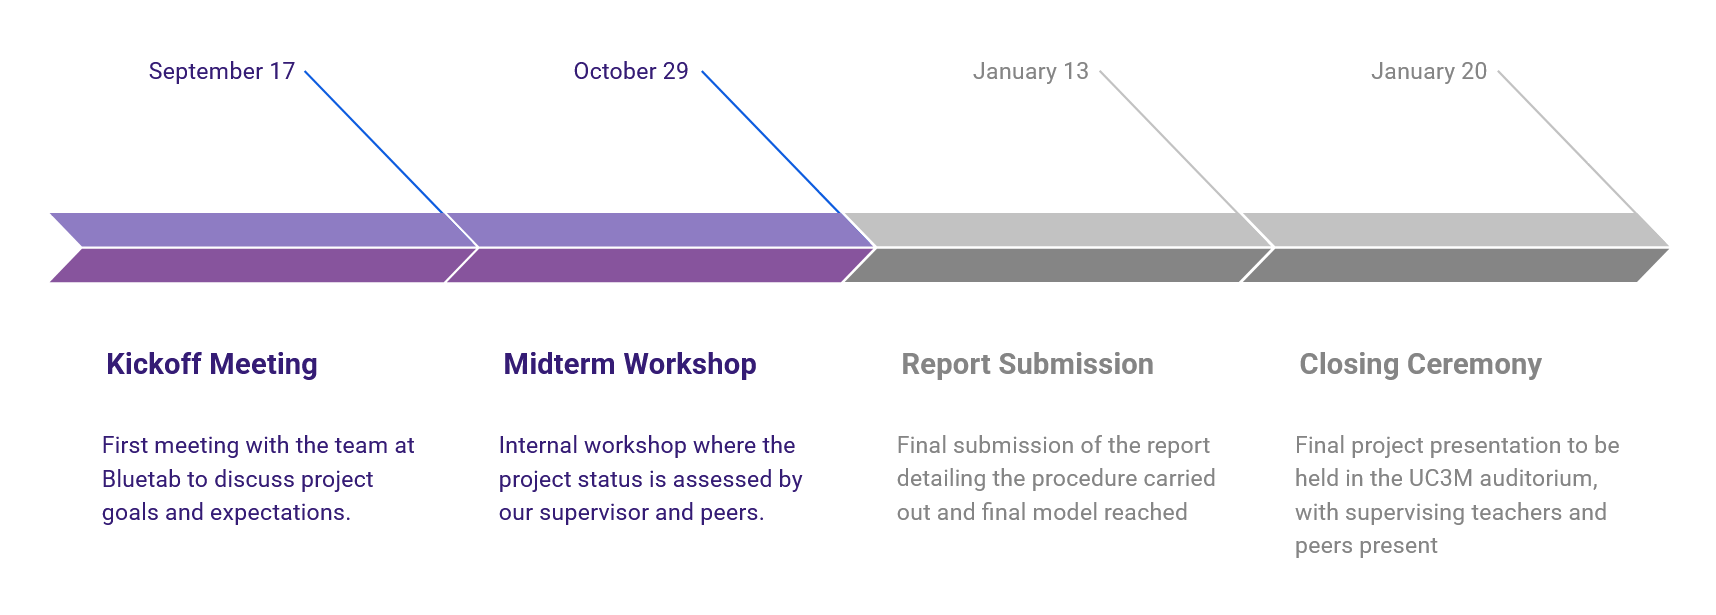
\includegraphics[width=1\textwidth]{Timeline.png}
    \caption{Project timeline.}
    \label{fig:timeline}
\end{figure}
\section{Background}
Nowadays, the modern financial system, including traditional and digital banks, as well as the insurance sector, operates in an environment of high complexity, which is regulated and characterized by a growing level of digital transactions.
The number of digital transactions has grown exponentially over the past few years, due to the facilities offered to customers worldwide when dealing with e-commerce, and being able to pay with our phones. But not everything is as good as it seems, as it has happened all over in the history of mankind; some people are willing to take advantage of those who are more vulnerable, who do not know someone who has not been targeted for a fraudulent action, such as identity theft, cloning the credit card, simulated transactions, money laundering or simply being catfished.

This represents a serious issue for financial entities, as they are currently operating on millions of daily transactions, for which just a small fraction of those could imply significant losses. That is why even though these transactions only represent 0.1 percent of the total volume, they can be equivalent to millions of dollars. This is the main reason why early and accurate detection is such an important and top-priority strategy.
\subsection{Most common fraud types}
For this project, instead of jumping directly on the data we were given, we decided to first understand the topic we were going to deal with for the past couple of months, so we did some research on which are the most common fraud types there are in the financial sector:
\begin{itemize}
    \item Credit Fraud: unauthorized access or cloning of credit/debit cards. 
    \item Identity Fraud: opening accounts or requesting credit access by means of false personal data.
    \item Internal Fraud: done by employees or partners.
    \item Money Laundering: complex movements to occult the illicit origin of the money. 
    \item Transaction Fraud: the one we are more interested in, account manipulation, or being tricked, such as phishing.
\end{itemize}

As each type has its own different patterns, the Machine Learning models must be able to detect anomalies for every context, such as the amount, the location, the schedule, or the client.
\subsection{Regulation and obligations}
We did not want to only focus on the basics, as we are expected to return not only a suitable model that is able to detect fraudulent transactions, but also we are committed to developing a design on Risk Management and Prevention Strategies based on what we have obtained during the project. That is why we have also done some research on how the financial sector is regulated and what legal obligations they must comply with. And what we have discovered is something we could think of, knowing that millions of dollars are at risk on a daily basis, it is a strong and well-regulated environment, in which the institutions must comply with international laws, such as :
\begin{itemize}
    \item KYC (Know Your Customer): Identification and verification of customers
    \item AML( Anti-Money Laundering): money laundering prevention
    \item Open Banking(only in Europe): API security and reinforced authentication
\end{itemize}
This implies that the fraud detection systems not only must be precise, but also be explicable and auditable. The transparency of the ML models is a technical and normative must-have.

\subsection{Technological Environment}
We also studied what the state-of-the-art was that the financial institutions have been adopting in recent years:
\begin{itemize}
    \item Real-time analysis systems based on Big Data
    \item ML models and the use of Deep Learning for detecting anomalies 
    \item Hybrid architectures( on-premise + cloud), for security and scalability
    \item Incorporating analytic dashboards for executive monitoring 
\end{itemize}

For the project team, being familiar with this new environment implied understanding that the technical decisions are conditioned by the laws and regulations, the cybersecurity, and the criticality of the financial operations.

\section{Business Impact}
The financial fraud has a direct impact on the profitability, the reputation, and the clients' trust. Based on industry studies, the cost of the fraud is estimated to represent between 0.5 and 1 percent of the total earnings of an entity. Furthermore, for each dollar lost due to fraud, businesses spend over 2 or 3 additional dollars in recuperation, investigation, and compensation processes.
This is the main reason why an intelligent detection system is not only a better technique, but also a strategy for reducing the losses, operational optimization, and law compliance.

\subsection{Main impacts}
\begin{itemize}
    \item Reduction of economic losses
    \begin{itemize}
        \item An efficient predictive model could be able to detect up to 80-90 percent of fraudulent transactions, cutting the losses.
        \item It also allows to detect the False Positives, those operations labeled as fraudulent when indeed they are not, reducing misunderstanding with the customers.
    \end{itemize}
    \item Improvement on the operational efficiency
    \begin{itemize}
        \item When automating the task classification, the workload of the human analyst is being reduced, which allows them to focus on the most critical cases
        \item This implies saving in terms of time and money when monitoring transactions
    \end{itemize}
    \item reputations and law compliance
    \begin{itemize}
        \item The proactive detection enhances the company's image in front of the clients.
        \item An institution that keeps track of the risk, boosts confidence, and reduces fines.
    \end{itemize}
    \item Optimizing the decision-making
    \begin{itemize}
        \item With dashboards and graphs, entities are more capable of identifying trends, regions, or segments that represent a higher risk.
    \end{itemize}
\end{itemize}
Evaluating the business impact shows that a fraud detection system is not just a technical development, but a strategy that protects assets, optimizes resources, and reinforces the client's trust. 

\section{Working Methods}
\begin{itemize}
\item Team workflow
\item Meetings with Bluetab
    \begin{itemize}
    \item September 17, this was the first session where we got the opportunity to know the company we were going to be working for during this semester, know the methodology we were supposed to implement while working on this project, and how it is structured.
    \item September 24, in this second meeting, we presented our first route map and distribution of the workload of all the members of the team, we discussed how we were going to approach the project and the first weeks.
    \item October 1, in the third session, we were able to present our first results, which were the first raw data exploration of the datasets we were given the week before. We also discussed some issues we encountered while performing the data exploration.
    \item October 8, for this fourth session, we had already performed a more robust EDA on the four datasets, and we also merged the data as it was suggested in the previous session. Furthermore, we also implemented an EDA and some techniques from previous courses, such as Mutual Information or PCA.
    \item October 15, for this session, we did not have a meeting with the company, but kept in touch and discussed via email our issues and improvements on the code, such as SMOTE to overcome the data imbalance.
    \item October 23, this has been the last session where we have presented the last improvements we have accomplished so far, such as implementing the first raw classifier models.
    \end{itemize}

\end{itemize}



\chapter{Exploratory Data Analysis}

\section{Raw Data Exploration}

\subsection{Overview of the raw sources}
We were given \textbf{four raw datasets}, each providing different information regarding bank transactions. 
\begin{itemize}
    \item \textbf{creditcard.csv} – A \textbf{284,807 $\times$ 31} dataset which contains anonymized information 
    about individual credit card transactions with the following variables:

    \begin{center}
    \begin{tabular}{|l|l|p{8cm}|}
        \hline
        \textbf{Variable} & \textbf{Type} & \textbf{Description} \\
        \hline
        \textit{Time} & Numeric (continuous) & Seconds elapsed between the transaction and the first recorded transaction in the dataset. \\
        \hline
        \textit{V1 -- V28} & Numeric (continuous) & Anonymized features resulting from a PCA transformation of original data. \\
        \hline
        \textit{Amount} & Numeric (continuous) & Monetary value of the transaction in local currency. \\
        \hline
        \textit{Class} & Binary (0/1) & Target variable: 0 indicates a legitimate transaction while 1 indicates a fraudulent transaction. \\
        \hline
    \end{tabular}
    \end{center}

    \item \textbf{transactions\_dirty.csv} – A \textbf{286,315 $\times$ 33} dataset which contains the same variables 
    as the last dataset minus the time variable and including three unique identifiers:

    \begin{center}
    \begin{tabular}{|l|l|p{8cm}|}
        \hline
        \textbf{Variable} & \textbf{Type} & \textbf{Description} \\
        \hline
        \textit{transaction\_id} & String & ID of the observed transaction. \\
        \hline
        \textit{customer\_id} & String & ID of the bank customer linked to the transaction. \\
        \hline
        \textit{device\_id} & String & ID of the device used to perform the transaction. \\
        \hline
    \end{tabular}
    \end{center}

    \item \textbf{locations\_dirty.csv} – A \textbf{286,315 $\times$ 6} dataset which includes geographical and merchant variables 
    for each transaction in addition to the transaction identifier:

    \begin{center}
    \begin{tabular}{|l|l|p{8cm}|}
        \hline
        \textbf{Variable} & \textbf{Type} & \textbf{Description} \\
        \hline
        \textit{ip\_address} & String & IP address associated with the transaction. \\
        \hline
        \textit{country} & Categorical & Country where the transaction occurred. \\
        \hline
        \textit{city} & Categorical & City where the transaction occurred. \\
        \hline
        \textit{zip\_code} & Categorical & Postal code of the transaction location. \\
        \hline
        \textit{merchant} & Categorical & Merchant's name. \\
        \hline
    \end{tabular}
    \end{center}

    \item \textbf{customers\_dirty.csv} – A \textbf{1,000 $\times$ 8} dataset which contains customer information 
    within the following variables, including the customer identifier:

    \begin{center}
    \begin{tabular}{|l|l|p{8cm}|}
        \hline
        \textbf{Variable} & \textbf{Type} & \textbf{Description} \\
        \hline
        \textit{name} & String & Customer's name. \\
        \hline
        \textit{age} & Numeric & Customer's age. \\
        \hline
        \textit{email} & String & Customer's email address. \\
        \hline
        \textit{phone} & String & Customer's phone number. \\
        \hline
        \textit{country} & Categorical & Customer's country of residence. \\
        \hline
        \textit{credit\_score} & Numeric & Customer's creditworthiness score. \\
        \hline
        \textit{join\_date} & Date & Date when the customer opened the account. \\
        \hline
    \end{tabular}
    \end{center}
\end{itemize}
    
\subsection{Variable grouping}
Having these four initially separated datasets provided a \textbf{clearer and more structured understanding} of the data landscape we were dealing with. This allowed us to understand the \textbf{role and relevance} of each variable and group them into different categories.
\begin{itemize}
    \item \textbf{Transactional} \\
    Formed by \textit{time}, \textit{amount}, and the 28 anonymized components (\(V1\)--\(V28\)).

    \item \textbf{Identifiers and keys} \\
    In this group we find the \textit{transaction\_id}, \textit{customer\_id}, and \textit{device\_id}. 
    These variables will be crucial for later dataset aggregation and leakage control in model evaluation.

    \item \textbf{Geolocation and merchant attributes} \\
    This group includes categorical fields with moderate to high numbers of categories such as 
    \textit{ip\_address}, \textit{country}, \textit{city}, \textit{zip\_code}, and \textit{merchant}. 
    They help describe the merchant context of each transaction and keep track of the “normal” behavior of customer transactions.

    \item \textbf{Customer attributes} \\
    Formed by variables such as \textit{age}, \textit{country}, and \textit{credit\_score} which help group customers due to their risk potential, 
    \textit{join\_date} that provides recency information, and contact fields like \textit{email} and \textit{phone} which might not seem useful at first; 
    however, their missingness can flag data-entry patterns.
\end{itemize}

\subsection{Univariate and bivariate characteristics}
To better understand the \textbf{statistical behaviour} of individual variables and the relationship between them we performed both univariate and bivariate examinations. The univariate analysis helped us study the \textbf{distribution} of each feature, which allowed us to identify skewed variables, potential outliers, and the need for normalization or transformation. On the other hand, the bivariate analysis focused on \textbf{relationships} between each variable and the target, which could help us recognize potential patterns and dependencies.

After performing univariate analysis for all numerical features we observed the following conclusions. The \textit{amount} is highly right-skewed meaning most of the transactions are of low quantity with a long tail extending to high quantity. The \textit{age} shows a relatively uniform distribution, which indicates a balanced representation of all age groups. The \textit{credit\_score} displays a bell-shaped distribution with values concentrated between 500 and 850 points, which represents a realistic distribution. Finally, the PCA-like variables \(V1\)--\(V28\) show approximately symmetric and centered distributions around zero, some being more dispersed than others, yet in accordance with standardized transformations having mean and variance around 0 and 1 respectively.
\begin{figure}[H]
    \centering
    
\includegraphics[width=1\textwidth]{univariate_numeric.png}
    \caption{Distribution of numeric features.}
    \label{fig:univariate_numeric}
\end{figure}
For the categorical features we highlight the following. The customer’s \textit{country} shows a highly long-tailed distribution including a large number of countries with very different frequencies, a small group dominating the dataset and the rest of countries appearing with progressively smaller counts. Unlike the latter, the merchant’s \textit{country} distribution shows a small number of countries with equal frequencies across the dataset, appearing to be balanced and uniform. Similarly, \textit{city} displays a semi-uniform distribution, counts being relatively even. Finally, the distribution of \textit{zip\_code} is relatively uniform, suggesting most zip codes occur at similar frequencies.
\begin{figure}[H]
    \centering
    
\includegraphics[width=1\textwidth]{univariate_categorical.png}
    \caption{Distribution of categorical features}
    \label{fig:univariate_categorical}
\end{figure}

To study the bivariate relationships we plotted the variables against the target \textit{Class}. From them we highlight that the fraudulent transactions tend to appear more around lower monetary values. For the rest of the variables only minimum differences between classes are shown. This analysis suggests that even though the classes appear to behave the same across most features, we might be facing a big imbalance problem in the target variable which could be misleading our conclusions.

\subsection{Class imbalance}
From our dataset we observe \textbf{284,068 non-fraudulent} entries (\textit{Class} = 0) and \textbf{2,000 fraudulent} entries (\textit{Class} = 1), resulting in a fraud rate of 0.7\%.Therefore, we conclude that \textit{Class} is severely imbalanced.
We will have to fix this problem in the following stages of our exploration in order to accomplish accurate and realistic classification results. One of the main solutions we contemplate is to use the library SMOTE to create synthetic data entries from the ones we already have.


% RAW DATA EXPLORATION - 2 pags aprx (3-4 mins) 
% Explicar los cuatro datasets 
% Las variables que tienen
% Distribuciones/ Univariate y Bivariate
% Class Imbalance

\section{Data Merge}
After analyzing each dataset, we decided to merge them in order to work with them. Before merging, we identified and solved inconsistencies that could compromise data integrity. In particular, we detected duplicated transaction\_id, which we carefully reviewed and cleaned removing those where its client\_id did not exist in customers\_df. This avoided null joins and ensured correct data merging. 
After merging, we performed a quick exploratory data analysis on the unified dataset. During this process, we standardized column names and adjusted variable data types (for instance, ensuring that numerical variables were in the correct format and categorical ones were properly encoded).
As mentioned above, an important observation was the severe class imbalance in the target variable. This imbalance is typical in fraud detection problems and has a direct impact on model evaluation.


\subsection{Missing values, Correlations and Outliers}
The next step was to perform a missing value analysis, which revealed some null in three columns related to the customer’s information. As it can be observed in Figure 2.1, these columns are: zip\_code, email, phone. To preserve all records, we imputed missing categorical values with the placeholder "Unknown", ensuring that these cases remained distinguishable but usable during training.
\begin{figure}[H]
    \centering
    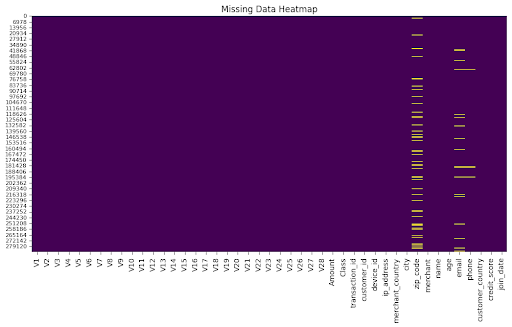
\includegraphics[width=0.8\textwidth]{missing_values.png}
    \caption{Location of missing values for each feature.}
    \label{fig:missing_values}
\end{figure}

Next, we examined variable correlations. The correlation heatmap showed that the anonymized features V1–V28 had very low pairwise correlations, which led us to think they were principal components. In addition, the contextual variables Amount, age, and credit\_score also displayed low correlation with the V-features, suggesting they provide complementary insights about each transaction.
Since no strong correlations were observed, we don’t have multicollinearity problems, which is beneficial for model training.
We also studied the correlation of each variable with the target (Class) to identify potential predictors of fraud. We studied the correlation plots, confirming that a few anonymized features were moderately associated with the target, while most had weak but non-zero relationships.
Finally, we conducted an outlier analysis, computing the number of outliers per variable with the IQR technique. Outliers were mostly concentrated in numerical features, reflecting the presence of unusually large or small transaction amounts, which can be meaningful indicators of fraudulent activity.

\subsection{PCA, Mutual Information and MRMR Analysis}
To deeply understand the data structure, we performed Principal Component Analysis as an exploratory step. PCA did not improve separability, which aligned with the idea of numerical variables coming from a given PCA. This confirmed that the dataset’s dimensionality is high, meaning multiple variables contribute small but complementary information.
We then computed the mutual information (MI) between each numerical feature and the target variable Class. Mutual information quantifies the dependency between variables and the target, regardless of linearity. The resulting MI ranking revealed that some features, particularly those among V10, V12, V14, and V17, hold the strongest dependency with the target. This aligns with results observed later in model-based feature importance analysis.
Additionally, we applied the Minimum Redundancy Maximum Relevance (MRMR) method to validate the MI results. MRMR selects features that are both highly relevant to the target and minimally redundant with each other. The consistency between MI and MRMR rankings confirmed the robustness of these top features.

\subsection{Model-Based Feature Selection}
To improve our understanding of feature relevance, we trained three tree-based ensemble models: XGBoost, LightGBM, and CatBoost.

The XGBoost model identified V14, V10, V12, and V17 as the dominant predictors, followed by V4, V8, and V20. Contextual variables like Amount, Age, and Credit Score had low importance scores. This confirms that the anonymized features contain most of the discriminative power for fraud detection.

In LightGBM, feature importance was measured by frequency of use in decision splits. The top-ranked features were V4, V26, V22, and credit\_score, followed by V15, V25, and V10. Interestingly, in contrast to XGBoost and CatBoost, credit\_score appeared among the most relevant variables, suggesting that its nonlinear interactions might be better captured by LightGBM’s leaf-wise growth strategy.

The CatBoost model, known for its strong performance on categorical and imbalanced data, highlighted V1, V4, V14, and Amount as top contributors. Once again, features like V12, V17, and V18 were also significant. Contextual features (age, credit\_score) remained relatively unimportant compared to the anonymized transaction components.

To sum up, we observed that features V10, V12, V14, and V17 were consistently high in importance. This internal consistency across algorithms reinforces the reliability of these features for fraud detection. 
These analyses were performed without any preprocessing, class balancing, or feature engineering, as the goal was purely exploratory. Nevertheless, the models achieved high accuracy, due to the extreme class imbalance, since it is predicting almost everything as ‘non-fraudulent’. 


\subsection{SMOTE}

Given the heavy class imbalance, we applied SMOTE to create a balanced dataset. SMOTE generates synthetic examples of the minority class (fraudulent transactions) by interpolating between existing minority samples. This approach helps models learn the characteristics of fraud without overfitting or losing valuable information from the majority class.

The balanced dataset obtained through SMOTE will be the foundation for the next modeling phase, where advanced preprocessing, feature engineering, and model evaluation with balanced metrics will be conducted.

% DATA MERGE: - 2 pags aprox 
% Cómo juntamos los datasets
% Missing values/ outliers/ correlations
% PCA/ Mutual information
% Modelos para feature selection
% Smote


\chapter{Next Steps and Future Work}

After finishing the phases of data integration, cleaning, and exploratory data analysis that have been explained in previous sections, the project is now entering into a new stage. It constitutes an intermediate milestone within the overall workflow, focused on deeper preprocessing, feature selection and, later on, advancing towards classification modelling. 

So far, the team has successfully built a consistent dataset from the original sources and has managed the class imbalance using SMOTENC. This consolidated data foundation will now support the enrichment of variables and the training of robust models capable of identifying fraudulent transactions efficiently. Some preliminary algorithms, which include XGBoost and LightGBM,  have already been tested, to obtain an initial performance baseline before more advanced preprocessing is applied.

The next step will be focused on advanced preprocessing and feature engineering. This includes transforming numerical variables, applying feature selection techniques, trying different encoding methods for the categorical variables and creating new features that capture more complex transactional patterns. Based on the insights we have obtained so far, the team has decided to place particular attention to temporal relationships, like time since the last transaction or spending trends, and to the behavioral anomalies through aggregated customer indicators (for example, transaction frequency or unusually high spending). These indicators are expected to reveal the fraudulent activities.

As an example of what we want to develop, the following table shows some of the ideas we have discussed for creating new variables during the feature-engineering process: 

\begin{table}[ht]
\centering
\begin{tabular}{|p{4cm}|p{4cm}|p{7cm}|}
\hline
\textbf{New Feature Idea} & \textbf{Based on} & \textbf{Purpose / Expected Insight} \\
\hline
transaction\_hour,\newline transaction\_day & time & Identify daily or weekly spending habits that may indicate rare behavior.\\
\hline
time\_last\_transaction& transaction\_id, time & Detect unusual gaps in transaction activity for each customer.\\
\hline
avg\_amount\_customer& customer\_id, amount & Measure the average spending per customer to flag unusually high transactions. \\
\hline
country\_mismatch & customer\_country, transaction\_country & Highlight transactions made from unexpected or new locations. \\
\hline
merchant\_risk\_rate & merchant, Class & Historical fraud rate per merchant; helps identify high-risk entities. \\
\hline
\end{tabular}

\end{table}


These variables are still a prototype and may evolve as the data exploration continue, but they represent the type of information that we are expecting to obtain after the feature engineering in order to make the classifier more accurate.

Another important aspect will be improving the pipeline to ensure reproducibility and efficiency. At the moment, all the functions are still on a single script, but the idea is to create an automated pipeline that consolidates preprocessing, feature engineering and resampling. This structured workflow will improve clarity and consistency, while also making it easier to adapt and deploy the model in the future.

In the upcoming weeks, the project will move towards the exploration and evaluation of classification models. This will involve training several binary supervised classifiers, such as CatBoost and XGBoost, and checking their performance through cross-validation, hyperparameter tuning and threshold selection. This phase is necessary to achieve a good balance between fraud detection and avoiding too many false alarms. To carry out this section, the group will need to research which models are the most suitable for fraud detection activity and the best metrics for their evaluation.

Once the final classifier is developed, the group will focus on optimization, fine-tuning and interpretability. In order to achieve a configuration that maximizes the detection accuracy while minimizing false positives, in order to work correctly in a real financial environment. As interpretability and transparency are truly relevant, some explainability techniques (like SHAP) will be implemented to understand the contribution of each feature in the final classification.

In addition, the visualization and dashboarding phase will be carried out. Their goal is to facilitate interpretation and communication of results by designing an interactive dashboard where the data distributions, temporal evolution alerts, and model behavior will be shown. It has both analytical and communication purposes, enabling non-technical stakeholders or people not involved in this project to understand the insights and outcomes obtained. 

One of the most important tasks comes at the end of this project, which is the design of strategies and recommendations. This is also one of the most challenging steps because it is an area we are not yet fully familiar with. However, it is essential for translating our results into practical decisions, as in a real project where the idea is not only to analyze the problem and obtain an algorithm, but to use that knowledge taking into account other areas such as financial impact and business perspective. Our team will propose some prevention and risk management measures, such as real-time alerts for suspicious transactions and fallback actions when risk is detected. Furthermore, we will estimate the possible business impact and return on investment (ROI) of implementing the proposed system, in order to reduce financial losses and improve the use of resources through simulated scenarios. This will be our first business impact assessment, giving us the chance to learn about the real economic and business effects of our project.

In summary, these steps represent the roadmap for the project in the following months to develop a robust and effective fraud detection system.


% \section{Feature Engineering}

% \section{Preliminary Models}

% \section{Fine Tuning and Gridsearch}


% IMPORTANT: Latex special characters are: # $ % & \ ^ _ { } ~. To avoid mistakes when compiling try writing \ before. For: \ use \textbackslash ; for ^ \textasciitilde and ~ \textasciicircum.

%     Example of figure:
%     \begin{figure}[H]
%     	\ffigbox[\FBwidth] {
%     	\caption[Name as seen in Index]{Figure name}
%     	}
%     	{
\includegraphics[scale=0.6]{imagenes/creativecommons.png}}
%     \end{figure}
    

\chapter{Conclusions}

Working on this project is a very rewarding experience for the team. Collaborating with Bluetab has given us the opportunity to experience working for a company, applying the knowledge obtained during the degree to a professional environment. Specifically, we are learning how machine learning techniques and data analysis are used in the financial sector, resulting in a really interesting experience as it is an area we had not explored in depth before.

We have faced and will keep facing new challenges and problems that help us grow both technically and professionally. Through this project, we are realizing the importance of having a clear workflow, documenting our progress properly, organizing our code and making the project easy to understand for all team members and the company. It is a long-term project, different to academic assignments we usually do, and it requires more coordination between us. Moreover, since we are not working with data that we have chosen and for which there is no predefined solution, as in university projects, the process is more demanding but also allows us to learn more and to face problems more similar to our professional future. Another key aspect is that we are not only developing a technical analysis or algorithm, we are also going to learn to interpret the results in a business context. This is a new and exciting challenge, which shows the practical value  and importance of data science in situations close to real-world problems and how it goes beyond simply building the model and observing results.

In addition, working with Bluetab is helping us improve our teamwork and communication skills. The weekly meetings with them have been very useful for us, they are highly committed and enthusiastic about the project, and they are always available for solving doubts and giving feedback. The team is truly grateful for the guidance and support we are receiving from them, which is making the learning process more structured and much easier. 

Overall, the experience of working with Bluetab is turning out to be very rewarding. We feel that we are learning a lot, improving our analytical and organizational skills, and becoming more confident in our contributions to business projects. It is satisfying to see how concepts studied at the university can be applied to problems closely related to real-world situations, and we are enthusiastic about continuing the development of our work in the next stages and dealing with new challenges. 



%----------
%	Bibliography
%----------	

%\clearpage
%\addcontentsline{toc}{chapter}{Bibliography}

% \printbibliography



%----------
%	Appendix
%----------	

% If your work includes Appendix, you can uncomment the following lines
%\chapter* {Appendix x}
%\pagenumbering{gobble} % Appendix pages are not numbered



\end{document}